\documentstyle[12pt,epsf]{article}


%\pagestyle{empty}
\parindent 0pt
\parskip 5mm

% declarations for front matter

\begin{document}
\begin{titlepage}




\begin{center}
{\LARGE \sc Geometry Description for MCFast}\\
\end{center}

\begin{abstract}
This document contains a description of MCFast geometry structures and
geometry files.    
\\

\end{abstract}
\begin{center}
MCFast v4\_3 and above \\
\today\\
\end{center}
\end{titlepage}

\tableofcontents

\section{MCFast Geometry Description}

The basic geometry shapes recognized by MCFast are planes, cylinders and cones. They can
be combined to form detectors elements such as silicon trackers, drift chambers, and
calorimeters.  Detectors other than silicon devices are generally described by the outer
box and the detector volume inside.  Materials are included  as either thin scatterers
or as thick absorbers.   Beam pipes and magnets are included as separate elements.

The detectors are assumed to be in regions of constant field.  
Magnets can be solenoids and dipoles.   Detector elements and magnets are described in
simple ASCII geometry files.  The expected formats of the files and a brief description
of the input is given in this document. 

MCFast tracking currently converts detector layers and scatterers into infinitely thin
planes or cylinders.  They are put into two ordered lists or radial planes and
$Z$-planes.  (See the routine 
\$MCFAST\_DIR/src/geom/geo\_trkorder.F).   
The calorimetry is the only part of MCFast that is volume based.   MCFast can handle
two tracking elements that are at the same radius or at the same $z$ position.  
MCFast allows does not check for overlapping volumes or planes, however, so be careful when
defining your detector.  

Geometry files in the DBin format are identified by the file extension {\it .db}.
Examples of MCFast geometry files can be found in \$MCFAST\_DIR/examples/mcfast. 
%
(To define \$MCFAST\_DIR {\it setup mcfast}.)
%


The geometry input variables are defined by templates.  
The template definitions for the various geometry geometry can be found in 
\$MCFAST\_DIR/db.  A link to \$MCFAST\_DIR/db must be made
inside the local directory where
you plan to run MCFast.  (ln -s \$MCFAST\_DIR/db db)  

Some geometry structures are nested which is defined in the
templates by a parent/child relationship.  The silicon barrel detector,
for example, has several levels: barrel detector elements, layers and wafers. 
Because we are working in fortran, the maximum number of elements is defined
inside the template.  If you exceed this number, strange things may happen.

This can be a confusing point.  The maximum number in the template is the 
total number of that element that can be defined in the detector.  There is
also a maximum number that is allowed per layer or per device that is defined 
internally to MCFast.  For ordinary non-nested structures, these numbers should
be the same.  For nested structures, these numbers are different and have been
set to reasonable values as determined by the authors.  These
numbers as they are implemented in the v2.6 version are given below.  

\subsection{Changing a MCFast Geometry Template}

If you would like to increase this number then you will need to contact one
of the authors or you can make your own version of MCFast libraries and 
change the template files yourself.  Remember that the geometry structures
are defined in the template files and separately in the include files.  
The geometry input is read in through condensed structures defined 
in the templates, and MCFast itself uses similar but less condensed
structures which can be found in \$MCFAST\_DIR/inc/geom.  The translation between the two
structure formats is done in the
\$MCFAST\_DIR/src/geom load\_*.F routines.  Since we are currently using Fortran,  
the maximum size of the arrays must be set for both structures.  We
have had to do this in two separate places which can cause problems when
something needs to be changed. 

{\bf For experts and the very brave}
To change a template yourself, you will need to
make your own copy of the mcfast files and have set the 
environment variable MCFAST\_DIR to your new directory.  
In \$MCFAST\_DIR/src/dbin\_mcfast you will find the main template file (template.db) and the
code that is auto-generated by dbin.  Create a link in this directory to the directory
containing your new template: ln -s \$MCFAST\_DIR/db db. 
Once you have changed the template
in \$MCFAST\_DIR/db and checked it against the corresponding fortran include file, 
run \~bphyslib/util/dev/dbin template.db.  You should now rebuild all MCFast libraries
and object files to be certain that there is no mismatch of version.     

 
\subsection{Units}

Mcfast uses standard units of cm, ns, grams, GeV and Tesla.  Angles are in radians.

\filbreak

\section{MCFast Geometry Input}

\subsection{Absorber}

The Absorber geometry structure describes cylindrical and conical inactive material.  Absorbers are treated in 
two ways inside MCFast.  Thin absorbers (type 41,42) are treated as scattering
sites and NO showers will be initiated inside them.   In v2\_6 thick absorbers are treated as
calorimeters without readout and showering can occur.  (See EMCAL structures.)  In v2\_5\_1
they are included in the graphics and the muon\_offline code.  

\begin{description}
\item[{\rm template} Absorber] (Max=25)  thick absorbers or thin scatterers(cylindrical/conic)
\begin{description}
\item[{\rm char} name]       name
\item[{\rm char} shape]     ``TUBE'' or ``CONE''
\item[{\rm int} type]        1=barrel, 2=forward, 41= barrel scatterer, 42= forward scatterer
\item[{\rm real} rmin(2)]    minimum radius at low z, high z
\item[{\rm real} rmax(2)]    maximum radius at low z, high z
\item[{\rm real} z0]         z at center
\item[{\rm real} zlen]       length in z
\item[{\rm material} material]  from material list
\end{description}
\item[end template]
\item[include file]  \$MCFAST\_DIR/inc/geom/absorber.inc, absorber\_struct.inc 
\end{description}


The AbsorberBox (new in v2\_6) geometry structure describes rectangular inactive material.  Absorbers are treated in 
two ways inside MCFast.  Thin absorbers (type 41,42) are treated as scattering
sites and NO showers will be initiated inside them.   Thick box absorbers are treated as
calorimeters without readout and showering can occur.  (See EMCALBox structures.)  

\begin{description}
\item[{\rm template} AbsorberBox] (Max=25)  thick absorbers or thin scatterers(cylindrical/conic)
\begin{description}
\item[{\rm char} name]       name
\item[{\rm char} shape]     ``BOX'' only
\item[{\rm int} type]        2=forward, 42= forward scatterer
\item[{\rm real} xlimit(2)]  xmin, xmax
\item[{\rm real} ylimit(2)]  ymin, ymax
\item[{\rm real} xlimit\_gap(2)]  inner gap xmin, xmax
\item[{\rm real} ylimit\_gap(2)]  inner gap ymin, ymax
\item[{\rm real} z0]         z at center
\item[{\rm real} zlen]       length in z
\item[{\rm material} material]  from material list
\end{description}
\item[end template]
\item[include file]  \$MCFAST\_DIR/inc/geom/absorber.inc, absorber\_struct.inc 
\end{description}

\filbreak
\subsection{Beampipe}

The beampipe is treated as a scatterer.  

\begin{description}
\item[{\rm template} BPipe](Max=2)  beam pipe (cylindrical)
\begin{description}
\item[{\rm  char} name]    name
\item[{\rm  real} rmin]    minimum radius (usually = 0)
\item[{\rm  real} rmax]    radius of inner wall
\item[{\rm  real} z0]      z at center
\item[{\rm  real} zlen]    length in z
\item[{\rm  material} mat\_fill]  fill material (``VACU'' for example)
\item[{\rm  real} bndrthk(4)]   wall thickness at rmin, rmax, front, back
\item[{\rm  material} matrbnd(4)] at rmin, rmax, front, back
\end{description}
\item[end template]
\item[include file] \$MCFAST\_DIR/inc/geom/beampipe.inc
\end{description}

\subsection{Detector}
This is where you will enter a general description of the detector including its name.  

\begin{description}
\item[{\rm template} detector]  Defines detector type for tracing
\begin{description}
\item[{\rm  char} name]  Detector Name
\item[{\rm  char} geom\_id]   Detector type  \\``CENTRAL'' cylindrical geometry
(solenoids)\\
``FORWARD'' z planes (dipoles)\\ ``COMBINED'' both  In early version of MCFast, this
was used to describe the geometry, now it simply serves as a switch for trk\_offline.  
Combined (wtk) fitting is much slower and is not very reliable.\\
\end{description}
\item[end detector]
\item[include file] \$MCFAST\_DIR/inc/geom/detector\_general.inc
\end{description}

\subsection{Dipole}

\begin{description}
\item[{\rm template} Dipole](Max=20)  Dipole magnets
\begin{description}
\item[{\rm  char} name]     name
\item[{\rm  real} bfield]   magnitude of B field
\item[{\rm  real} dircos(3)]  direction of b-field  (current version assumes 
fields along $x$ or $y$ axis)
\item[{\rm  real} xmin]  minimum x for field region 
\item[{\rm  real} xmax]  maximum x for field region
\item[{\rm  real} ymin]  minimum y for field region
\item[{\rm  real} ymax]  maximum z for field region
\item[{\rm  real} z0]    central value for z
\item[{\rm  real} zlen]  length of field region in z
\item[{\rm  material} mat\_fill]  fill material usually ``AIR''
\item[{\rm  real} thick\_boun(6)]  Yoke thickness at: xmin, xmax, ymin, ymax, zmin, zmax  
\item[{\rm  material} mat\_boun(6)]  Yoke material at: xmin, xmax, ymin, ymax, zmin, zmax
\end{description}
\item[end template]
\item[include file] \$MCFAST\_DIR/inc/geom/dipole.inc, dipole\_struct.inc
\end{description}

\filbreak

\subsection{Drift Chambers}  Central Drift Chamber (cylindrical)

\begin{description}
\item[{\rm template} Drift](Max=10)
\begin{description}
\item[{\rm  int} num]    Chamber number
\item[{\rm  char} name]  Name
\item[{\rm  int} num\_anode]  Number of anode layers
\item[{\rm  child} LayerDRFAno] Link to daughter structure  : no entry in .db file
\item[{\rm  child} OffsetDRFAno]  Link to daughter structure: no entry in .db file
\item[{\rm  int} num\_cathode]  number of cathode layers  (can be zero)
\item[{\rm  child} LayerDRFCatho]  Link to cathode structure
\item[{\rm  real} rmin]   minimum radius of drift volume
\item[{\rm  real} rmax]   maximum radius of drift volume
\item[{\rm  real} z0]     central Z position
\item[{\rm  real} zlen]   length of chambers
\item[{\rm  material} material]  fill material 
\item[{\rm  real} thick\_boun(4)]  boundary thickness at rmin, rmax, zmin, zmax
\item[{\rm  material} mat\_boun(4)]  boundary material rmin, rmax, zmin, zmax
\end{description}
\item[end template]
\item[include file] \$MCFAST\_DIR/inc/geom/drift.inc, drift\_struct.inc
\end{description}
Drift chamber substructure:
\begin{itemize}
\item Drift\_cathode
\begin{description}
\item[{\rm template} LayerDRFCatho](Max=2 total, max= 2 per device)  Drift Chamber Cathode (not used currently)
\begin{description}
\item[{\rm  int} det]       Pointer to parent Drift chamber
\item[{\rm  parent} Drift]  parent structure: no entry in .db file
\item[{\rm  int} lyr]       Cathode layer number
\item[{\rm  real} delta\_r] 
\item[{\rm  real} zlen]     cathode length in z
\item[{\rm  int} nstrips]   number of strips in z
\item[{\rm  int} n\_phi\_segm]  number of segments in phi
\item[{\rm  int} ID\_anode] points to corresponding anode layer 
\item[{\rm  int} cell\_offset] phi offset of strips
\item[{\rm  real} eff\_hit] efficiency
\item[{\rm  real} resa]    
\item[{\rm  real} resb]
\item[{\rm  real} resc]
\end{description}
\item[end template]
\item[include file] \$MCFAST\_DIR/inc/geom/drf\_cathode\_struct.inc
\end{description}
\item Drift\_layer
\begin{description}
\item[{\rm template} LayerDRFAno](Max=100 total, Max= 100 per device)
\begin{description}
\item[{\rm  int} det]   pointer to Drift chamber
\item[{\rm  parent} Drift] Parent Structure:  No entry in .db file
\item[{\rm  int} lyr]      Anode layer number
\item[{\rm  real} radius]  radius of layer
\item[{\rm  real} zlen]    length of anode
\item[{\rm  real} cell\_height]  height of cell
\item[{\rm  int }nwires]   number of wires in layer
\item[{\rm  int} ID\_readout]  readout side +1 = zmax, -1 = zmin
\item[{\rm  int} ID\_cathode]  cathode plan corresponding to this anode
\item[{\rm  real} phi0]  phi offset (phi of wire 0)
\item[{\rm  real} stereo\_tau]  
\item[{\rm  real} stereo\_offset]
\item[{\rm  real} eff\_hit]  hits efficiency 
\item[{\rm  real} eff\_dedx] efficiency for dedx info
\item[{\rm  real} siga]  $ \sigma = \sigma_a + \sigma_b \times drift + \sigma_c \times drift^2 $
$(drift = (drift time)/max(drift time)$
\item[{\rm  real} sigb]
\item[{\rm  real} sigc]
\end{description}
\item[end template]
\item[include file] \$MCFAST\_DIR/inc/geom/drf\_anode\_struct.inc
\end{description}
\item Drift\_offset
\begin{description}
\item[{\rm template} OffsetDRFAno](Max=100 total, Max = 100 per device)  Drift Chamber offsets (defaults to zero offset)
\begin{description}
\item[{\rm  int} det]  pointer to Drift chamber
\item[{\rm  parent} Drift]  Parent Structure: no entry in structure
\item[{\rm  int} lyr]  anode layer
\item[{\rm  real} cell\_offset]  
\item[{\rm  real} sag]
\item[{\rm  real} offset(3)]
\item[{\rm  real} dircos(3)]
\end{description}
\item[end template]
\item[include file] \$MCFAST\_DIR/inc/geom/drf\_anode\_struct.inc
\end{description}
\end{itemize}

\filbreak

\subsection{Electromagnetic Calorimeters}  

The basic Cylindrical Calorimeter Structure is called EMCal.  This will
serve as the model a new calorimeter structure that will be developed for future 
versions.  

\begin{description}
\item[{\rm template} EMCal](Max=40)
\begin{description}
\item[{\rm  char} name]   Name of calorimeter
\item[{\rm  char} shape]  Shape ``TUBE'' or ``CONE''
\item[{\rm  int}  type]   central (=1), forward or backward(=2)
\item[{\rm  real} rmin(2)]  minimum radius at lo z, hi z
\item[{\rm  real} rmax(2)]  maximum radius at lo z, hi z
\item[{\rm  real} z0]       central z position
\item[{\rm  real} zlen]     length in z
\item[{\rm  material} material]  average mixture of calorimeter material  
\item[{\rm  material} active]    active material
\item[{\rm  int} nphi]           number of segments in phi
\item[{\rm  int} neta]           number of segments in eta
\item[{\rm  real} siga\_em]      resolution for electromagnetic showers
\item[{\rm  real} sigb\_em]      offset for electromagnetic showers
\item[{\rm  real} siga\_had]     resolution for hadronic showers
\item[{\rm  real} sigb\_had]     offset for hadronic showers
\item[{\rm  real} em\_had\_ratio]  e/pi ratio 
\end{description}
\item[end template]
\item[include file] \$MCFAST\_DIR/inc/geom/emcal.inc, emcal\_struct.inc
\end{description}

The basic Boxlike Calorimeter Structure is called CalorBox (New in v2\_6).  

\begin{description}
\item[{\rm template} CalorBox](Max=40)
\begin{description}
\item[{\rm  char} name]   Name of calorimeter
\item[{\rm  char} shape]  Shape ``BOX'' only
\item[{\rm  int}  type]    forward or backward(=2)
\item[{\rm  real} xlimit(2)] xmin, xmax
\item[{\rm  real} ylimit(2)] ymin, ymax
\item[{\rm  real} xlimit\_gap(2)] inner gap xmin, xmax
\item[{\rm  real} ylimit\_gap(2)] inner gap ymin, ymax
\item[{\rm  real} z0]       central z position
\item[{\rm  real} zlen]     length in z
\item[{\rm  material} material]  average mixture of calorimeter material  
\item[{\rm  material} active]    active material
\item[{\rm  int} ncr1]           number of segments in x
\item[{\rm  int} ncr2]           number of segments in y
\item[{\rm  real} siga\_em]      resolution for electromagnetic showers
\item[{\rm  real} sigb\_em]      offset for electromagnetic showers
\item[{\rm  real} siga\_had]     resolution for hadronic showers
\item[{\rm  real} sigb\_had]     offset for hadronic showers
\item[{\rm  real} em\_had\_ratio]  e/pi ratio 
\end{description}
\item[end template]
\item[include file] \$MCFAST\_DIR/inc/geom/emcal.inc, emcal\_struct.inc
\end{description}


\filbreak

\subsection{Forward tracking}
\label{sec:ftrk}

\begin{description}
\item[{\rm template} FTrk](Max=100)   Forward tracking devices  -- Box-like
\begin{description}
\item[{\rm  int} det]    Detector number (1...100)
\item[{\rm  char} name]  Detector name
\item[{\rm  int} nlyr]   number of detection planes 
\item[{\rm  child} LayerFTRK]  detection plane structure  (no entry in .db file)
\item[{\rm  real} xmin]  xmin of the device
\item[{\rm  real} xmax]  xmax of the device
\item[{\rm  real} ymin]  ymin of the device
\item[{\rm  real} ymax]  ymax of the device
\item[{\rm  real} z0]    central z position
\item[{\rm  real} zlen]  length in z
\item[{\rm  material} mat\_fill]  fill material or gas mixture
\item[{\rm  real} thick\_boun(6)]   thickness of box at: xmin, xmax, ymin, ymax, zmin, zmax
\item[{\rm  material} mat\_boun(6)] material of box at:  xmin, xmax, ymin, ymax, zmin, zmax
\item[{\rm  real} siga] resolution
\item[{\rm  real} sigb]
\item[{\rm  real} sigc]  
\end{description}
\item[end template]
\item[include file] \$MCFAST\_DIR/inc/geom/for\_trk.inc, for\_trk\_struct.inc
\end{description}

\filbreak
Forward tracking layer structure:
\begin{itemize}
\item Ftrk\_layer\\
Detection planes for box-like forward chambers.
\begin{description}
\item[{\rm template} LayerFTRK](Max=500 total, max= 100 per device)
\begin{description}
\item[{\rm  int} det]  pointer to FTrk
\item[{\rm  parent} FTrk]  FTrk structure (no entry in .db file)
\item[{\rm  int} lyr]  layer number.  Layers must be numbered in
                       increasing order of z.
\item[{\rm  real} z\_local]   local z wrt to center of FTrk Box
\item[{\rm  real} thick]      thickness of detection layer 
\item[{\rm  real} xmin]       xmin of detection plane
\item[{\rm  real} xmax]       xmax of detection plane
\item[{\rm  real} xmin\_gap]  xmin of gap in detection plane
\item[{\rm  real} xmax\_gap]  xmax of gap in detection plane
\item[{\rm  real} ymin]       ymin of detection plane
\item[{\rm  real} ymax]       ymax of detection plane
\item[{\rm  real} ymin\_gap]  ymin of gap in detection plane
\item[{\rm  real} ymax\_gap]  ymax of gap in detection plane
\item[{\rm  real} stereo]     stereo angle 
                              ($[-\frac{\pi}{2},+\frac{\pi}{2},]$radians);
                              see text for details.
\item[{\rm  int} ncell]       number of cells
\item[{\rm  real} coord0\_x]  x coordinate of 1st cell
\item[{\rm  real} coord0\_y]  y coordinate of 1st cell
\item[{\rm  int} type]        controls interpretation of stereo; see text for 
                              details.
\item[{\rm  real} eff\_hit]   hit efficiency
\item[{\rm  real} siga]       $\sigma = \sigma_a + \sigma_b*(drift dist) + \sigma\_c*(drift dist)^2$;\\
if $\sigma=0$ , $\sigma = cell size / \sqrt{12}$
\item[{\rm  real} sigb]
\item[{\rm  real} sigc]
\end{description}
\item[end template]
\item[include file] \$MCFAST\_DIR/inc/geom/for\_trk\_lyr\_struct.inc
\end{description}
\end{itemize}

\filbreak
Inside MCFast it is assumed that, within one forward tracking detector,
the layer numbers are in increasing order of z.  
This is illustrated in figure~\ref{ftrk5}.  For experts only:
this assumption is made geo\_trkorder\_for\_trk.F when the position 
of the scattering surfaces between layers is computed.  The consequences
of violating the rule are relatively small: the scattering in the material
between layers occurs at the wrong value of $z$.
\begin{figure} [tbp]
\centerline{\epsfysize=1.5in \epsffile{ftrk5.eps}}
\caption{\label{ftrk5}  The rule for ordering layers within a 
forward tracking detector: layer 1 is at the lowest value of
$z$.  One consequence of this is that if an $xuv$ multiplet
is mirror-symmetric about $z=0$, the mapping of layer number
to view type is not preserved.  The labeling of the views in this figure
is for illustrative purposes only.  }
\end{figure}

Until MCFast v5\_0 the value of the {\tt type} element of
the ftrk template was undefined and was ignored by the code; there 
were some comments floating around which suggest that it once had
a planned use which was never implemented.
In MCFast v5\_0 the element {\tt type} was given
meaning; the different values of {\tt type} describe different
interpretations of the {\tt stereo} element of the ftrk template:
\begin{itemize}
\item {\tt type=1} The outer edges of the forward tracking plane and the
                   edges of the central hole are aligned
                   with the world $x$ and $y$ axes; the wires 
                   are strung at the specified angle within that frame.
                   See figures~\ref{ftrk1} and~\ref{ftrk2}. 
\item {\tt type=2} and {\tt type=3}. 
                   The wires are strung parallel to the edges of the
                   frame and the entire frame is rotated by the
                   specified angle.  The edges of the gap are parallel
                   to the edges of the frame.  See figures~\ref{ftrk3} 
                   and~\ref{ftrk4}.
\item All other values of {\tt type} are treated as {\tt type=1}.
\end{itemize}

Figure~\ref{ftrk1}, which illustrates {\tt type=1}, 
shows three rectangles.
% 
\begin{figure} [htbp]
\centerline{\epsfysize=3.0in \epsffile{ftrk1.eps}}
\caption{\label{ftrk1} Example of a type 1 silicon strip detector with 
a positive stereo angle.
}
\centerline{\epsfysize=3.0in \epsffile{ftrk2.eps}}
\caption{\label{ftrk2} Example of a type 1 silicon strip detector with 
a negative stereo angle.
}
\end{figure}
%
The outermost
rectangle represents the outer edge of the material which makes up
the forward tracking plane.  The innermost rectangle represents
the edges of the beam hole.  The mid-sized rectangle
represents the outer boundary of the
active region of the layer. The diagonal
lines represent several of the strips which fill the sensitive
area; the stereo angle is indicated on the figure and, for this example,
it is positive.  Notice that the strips are broken by the central
hole.  The ftrk template quantities {\tt xmin, xmax, ymin, ymax} 
are defined by large black dots on the outermost rectangle.  The
template quantities
{\tt coord0\_x and coord0\_y} are defined by the dot in the lower
left corner of the sensitive area; this point is labeled
$(x_0,y_0)$.  The coordinates of the upper right corner of the sensitive
area are not specified: to deal with this, the code assumes that the 
right-hand insensitive margin has the same width as the left-hand one; 
similarly, the code assumes that the upper insensitive margin has the 
same height as the lower one; that is, the active area is centered
on the full area of the layer.
Before MCFast v5\_0, there were bugs in the code which positioned the
active area on the full area; the bugs were not triggered if the active
area was the same size as the full area.
The quantities labeled $\vec{\eta}$ and
$(x_1,y_1)$ are only of relevance to very expert users and
to developers; they will be discussed at the end of this sub-section.

Figure~\ref{ftrk2} illustrates a configuration which has only
one difference from that shown in figure~\ref{ftrk1}: in this
case the stereo angle is negative.

Figure~\ref{ftrk3} illustrates a forward tracking plane
of type~2.  
%
\begin{figure} [htbp]
\vskip -2. cm
\centerline{\epsfysize=3.0in \epsffile{ftrk3.eps}}
\caption{\label{ftrk3} Example of a type 2 silicon strip detector with a
positive stereo angle.  The plane is oriented as shown in the right
hand figure but the size parameters are defined in the $\theta=0$ 
configuration shown to the left.  The rotation is made about the
$z$ axis.
}
\centerline{\epsfysize=3.0in \epsffile{ftrk4.eps}}
\caption{\label{ftrk4} Example of a type 3 silicon strip detector with 
a positive stereo angle.  This is distinguished from a type~2
detector by the orientation of the strips.
The plane is oriented as shown in the right
hand figure but the size parameters are defined in the $\theta=0$ 
configuration shown to the left.  The rotation is made about the
$z$ axis.
}
\end{figure}
%
The left part of the figure shows a plane when the stereo angle,
$\theta$, is zero. The quantities which define the size of the plane
are defined in this configuration; these quantities are,
{\tt xmin, xmax, ymin, ymax, coord0\_x} and {\tt coord0\_y}.
This is indistinguishable from a type~1 detector with $\theta=90^{\circ}$.
The configuration on the right hand side illustrates the detector
when $\theta$ is non-zero; in this case it is positive.  This differs
from a type~1 detector in that the entire detector, frame and all,
has been rotated.  For convenience, the parameters
 {\tt xmin, xmax, ymin, ymax, coord0\_x} and {\tt coord0\_y} are defined
in the $\theta=0$ configuration, even when $\theta$ has
a non-zero value.

Figure~\ref{ftrk4} illustrates a forward tracking detector
of type~3. This differs from a type~2 detector in the 
orientation of the wires.

There is no facility within MCFast to specify one rotation
angle for the frame and a different one for the wires.

The remaining material in this sub-section is for experts only.

In the last four figures there are items labeled
$(x_1,y_1)$ and $\vec{\eta}$.  These items are not found in the
template and only expert MCFast users need consider them.
They are used in the computation of the cell number of the hit cell
and in the computations of the parameters which describe
a hit.  To compute the cell number one needs a 
reference point, $\vec{x_0}$, and a measurement direction $\vec{\eta}$.
This direction lies in the plane of the detector and is perpendicular 
to the wire direction.  Given a point in the plane, $\vec{x}$, the
cell which contains the hit, $n$, is given by,
\begin{eqnarray}
n &=& {\rm int}\left( (\vec{x}-\vec{x_0})\cdot\vec{\eta}\right).
\end{eqnarray}
With an appropriate choice of $\vec{x_0}$, this gives values
of $n$ which lie between 0 and {\tt ncell-1}.  
Consider figure~\ref{ftrk2}.
In this figure the arrow labeled
$\vec{\eta}$ shows the sign convention for the
measurement direction and the point  
labeled $(x_0,y_0)$ is the unique point which satisfies all
of the requirements for the the reference point.  This
choice of reference point works for all negative stereo angles 
and for a stereo angle of zero.

Now consider figure~\ref{ftrk1}, which shows a positive stereo angle.
Again the arrow labeled $\vec{\eta}$
shows the sign convention for the measurement direction.
If the same reference point were chosen as for the case of a negative stereo
angle, then $n$ would take on negative values.  In order to avoid this,
MCFast internally changes the reference point to the point labeled 
$(x_1,y_1)$, at the upper left corner of the sensitive area.
This is strictly internal to MCFast and is out of control
of the user; the geometry file still
requires that the point $(x_0,y_0)$ be specified for
{\tt coord0\_x} and {\tt coord0\_y}.

Now consider figures~\ref{ftrk3} and ~\ref{ftrk4}.  In these cases
the measurement direction is parallel to one of the edges of the
detector and it rotates along with the plane.  The reference point
is the point $(x_1,y_1)$; these are the world coordinates of the
position to which the point $(x_0,y_0)$ is moved by the rotation.

Note, however, that the reference point which is stored in the
hit structure is neither $(x_0,y_0)$ nor $(x_1,y_1)$ --- it happens
to be a point on the hit wire.  The convention for that reference 
point will be described in another note.

One should notice that the cell size ( or pitch ) is not
a template parameter.  It is derived from the number of cells ({\tt ncell}),
which is a template parameter, and the size of the active area, which
can be inferred from the template parameters.  In all cases except for
that of
a type~1 layer with an arbitrary stereo angle, the computation of
the cell size is straightforward.
Figure~\ref{ftrk6} sets up the algebra for computing the cell size for
the non-trivial case.   The lower left-hand 
corner of the active region, point $A$, is at the lower edge of cell 0
and the upper right corner of the active region, point $D$ is at the
upper edge of cell {\tt ncell-1}.  The measurement direction is shown
twice as two thick, red lines marked $\vec{\eta}$. 
Some of the strips are drawn perpendicular to $\vec{\eta}$.  
The points $B$ and $C$ are on a line which is parallel to the strips 
and which goes through the lower right corner of the active region.   
The cell size is given by,
\begin{eqnarray}
{\tt cell\_size} &=& \frac{|AB|+|CD|}{\tt ncell} \nonumber \\
&=& \frac{|xdim\times\sin{\theta}| + | ydim\times\cos{\theta}|}
     {\tt ncell}
\end{eqnarray}
The figure shows the case that the stereo angle is less than zero but
the final result holds for all values of the stereo angle.
%
\begin{figure} [btp]
\centerline{\epsfysize=3.0in \epsffile{ftrk6.eps}}
\caption{\label{ftrk6}  Figure showing how to compute {\tt ncell} for
{\tt type=1} and a general stereo angle. The definition of
the stereo angle is shown in figures~\protect{\ref{ftrk1}}
and ~\protect{\ref{ftrk2}}.  See the text for details. }
\end{figure}


\newpage
\subsection{Hadron calorimeter}  

The Hadron calorimetry structure is now obsolete.  
%This structure will  be replaced by a unified
%calorimeter structure in v2.5.  For Snowmass use EMCal to describe your calorimeters if you 
%want to make EM and hadronic showers.  
  
%%\begin{description}
%%\item[{\rm template} HADCal](Max=1)  
%%Will be replaced in v2.5.
%%\begin{description}
%%\item[{\rm  char} name]
%%\item[{\rm  char} shape]
%%\item[{\rm  int} type]
%%\item[{\rm  real} rmin(2)]     ! lo z, hi z
%%\item[{\rm  real} rmax(2)]     ! lo z, hi z
%%\item[{\rm  real} z0]
%%\item[{\rm  real} zlen]
%%\item[{\rm  material} material]
%%\item[{\rm  int} nphi]
%%\item[{\rm  int} neta]
%%\item[{\rm  real} siga]
%%\item[{\rm  real} sigb]
%%\end{description}
%%\item[end template]
%%\end{description}

\subsection{Hits on track}  

Sets minimum number of hits required for an ``offline'' track

\begin{description}
\item[{\rm template} HitsOnTrack](Max=2)
\begin{description}
\item[{\rm  int} all]    Minimum number of hits required in track fit 
\item[{\rm  int} z]      Minimum number of stereo hits  --  USER cut only
\item[{\rm  int} svx]    Minimum number of silicon hits --  USER cut only
\end{description}
\item[end template]
\item[include file] \$MCFAST\_DIR/inc/geom/track\_minhit.inc
\end{description}

\filbreak

\subsection{Materials}   List of Materials and Mixtures
\begin{description}
\item[{\rm template} Material](Max=50)
\begin{description}
\item[{\rm  char} name]   Name
\item[{\rm  real} a]      A
\item[{\rm  real} z]      Z
\item[{\rm  real} density]  density  [g/cm$^3$]
\item[{\rm  real} radlen]   radiation length  [cm]
\item[{\rm  real} abslen]   absorption length [cm]
\item[{\rm  real} collen]   collision length  [cm]
\item[{\rm  real} dedx]     dedx [GeV/cm]
\end{description}
\item[end Material]
\item[include file] \$MCFAST\_DIR/inc/geom/material.inc,
material\_struct.inc
\end{description}

Example of a material list\\

\begin{tabular}{rclllllll}
         &  name   &      A      &    Z       &density    &RadLen     &AbsLen     &ColLen     & Dedx\\
Material & "VACU" &  0.1000E-15 & 0.1000E-15 & 0.1000E-15 & 0.1000E+17 & 0.1000E+17 & 0.10E+17 & 0.1000E-15\\
Material & "AIR"  &  0.1461E+02 & 0.7300E+01 & 0.1250E-02 & 0.3042E+05 & 0.6750E+05 & 0.10E+17 & 0.2190E-05\\
Material & "ALUM" &  0.2698E+02 & 0.1300E+02 & 0.2700E+01 & 0.8900E+01 & 0.3720E+02 & 0.10E+17 &0.4370E-02\\
Material & "IRON" &  0.5585E+02 & 0.2600E+02 & 0.7870E+01 & 0.1760E+01 & 0.1710E+02 & 0.10E+17 &0.1165E-01\\
Material & "SILI" &  0.2809E+02 & 0.1400E+02 & 0.2330E+01 & 0.9360E+01 & 0.3000E+02 & 0.10E+17 &0.3870E-02\\
Material & "SCIN" &  0.1200E+02 & 0.6000E+01 & 0.1032E+01 & 0.4240E+02 & 0.7940E+02 & 0.10E+17 &0.2010E-02\\
Material & "CU"   &  0.6354E+02 & 0.2900E+02 & 0.8960E+01 & 0.1430E+01 & 0.1030E+02 & 0.10E+17 &0.1290E-01\\
Material & "TITA" &  0.4790E+02 & 0.2200E+02 & 0.4540E+01 & 0.3560E+01 & 0.2750E+02 & 0.10E+17 &0.6850E-02\\
Material & "BE"   &  0.9010E+01 & 0.4000E+01 & 0.1848E+01 & 0.3530E+02 & 0.3670E+02 & 0.10E+17 &0.2970E-02\\
Material & "CARB" &  0.1201E+02 & 0.6000E+01 & 0.2265E+01 & 0.1880E+02 & 0.3820E+02 & 0.10E+17 &0.4030E-02\\
Material & "CFIB" &  0.1201E+02 & 0.6000E+01 & 0.2265E+01 & 0.2140E+02 & 0.4990E+02 & 0.266E+02 &0.4030E-02\\
Material & "MXSO" &  0.5572E+02 & 0.2550E+02 & 0.6026E+01 & 0.2372E+01 & 0.2481E+02 & 0.10E+17 &0.9875E-02\\
Material & "ARGON"&     39.95   & 18.0       & 1.78E-3    & 11706.     & 5.E+4      & 1.E+16   &2.70E-6\\
Material & "C2H6" &     30.8    & 18.0       & 1.36E-3    & 34035.     & 5.E+4      & 1.E+16   &3.05E-6\\
Material & "MIX1" &  0.5077E+02 & 0.2368E+02 & 0.4451E+01 & 0.3380E+01 & 0.3181E+02 & 0.10E+17 &0.1053E-01\\
\end{tabular}

\subsection{Mixtures}  Mixtures
\begin{description}
\item[{\rm template} Mixture](Max=20)
\begin{description}
\item[{\rm  char} name]            mixture name
\item[{\rm  int} nmat]             number of materials
\item[{\rm  material} matnames(5)]     material names
\item[{\rm  real} prop(5)]         proportion by volume
\end{description}
\item[end template]
\item[include file] \$MCFAST\_DIR/inc/geom/material.inc,
material\_struct.inc
\end{description}

\filbreak

\subsection{Muon}  Very Simple Muon Detector
In v2\_5\_1 the muon detector is completely separate from the tracking and the muon\_offline
code estimates the amount of absorber and calorimeter material the muon sees and does a
rough calculation of dedx.   In v2\_6 this will be more integrated into the tracking and
tracing code. 
\begin{description}
\item[{\rm template} MUON](Max=40)  cylindrical geometry
\begin{description}
\item[{\rm  char} name]
\item[{\rm  char} shape]   Shape ``TUBE'' or ``CONE''
\item[{\rm  int} type]        central = 1, forward or backward = 2
\item[{\rm  real} rmin(2)]    minimum radius at lo z, hi z
\item[{\rm  real} rmax(2)]    maximum radius at lo z, hi z
\item[{\rm  real} z0]         central z position
\item[{\rm  real} zlen]       length in Z
\item[{\rm  material} material]  average material (not used)
\item[{\rm  int} nlayer]      number of layers
\end{description}
\item[end template]
\item[include file] \$MCFAST\_DIR/inc/geom/muon.inc, muon\_struct.inc
\end{description}

\filbreak

\subsection{Silicon barrel detectors}
\label{page:sib:detectors} Silicon barrel detectors
are described as collections of planar wafers that are positioned
such that their normal vector is in the $xy$ plane.
See figures \ref{sib1} and \ref{sib2}.  For
purposes of tracking the wafers are treated as
infinitesimally thin objects.  However the description of the
wafer does include a thickness, which is only used
in the computation of the expected multiple scattering and energy loss;
these are applied as if they occured at the infinitesimally thin plane.
Also, the quantity $\beta$ in the db file is not the same as the
$\beta$ which appears in the include file; see figure~\ref{sib2} and
the discussion about include files, which begins on 
page~\pageref{page:sib:include}.  
Finally, figure~\ref{sib3} gives a
graphical representation of the connections between the components of
the silicon barrel description.

\begin{description}
\item[{\rm template} SiBarrel](Max=15)
\begin{description}
\item[{\rm  int} num]
\item[{\rm  char} name]
\item[{\rm  int} nlyr]
\item[{\rm  child} LayerSiB]
\item[{\rm  real} z0\_global]  central z position for detector
\end{description}
\item[end template]
\item[include file] \$MCFAST\_DIR/inc/geom/si\_barrel.inc, 
si\_barrel\_struct.inc 
\end{description}

\begin{figure} [htbp]
\centerline{\epsfxsize=5.0in \epsffile{sib.eps}}
%\centerline{
%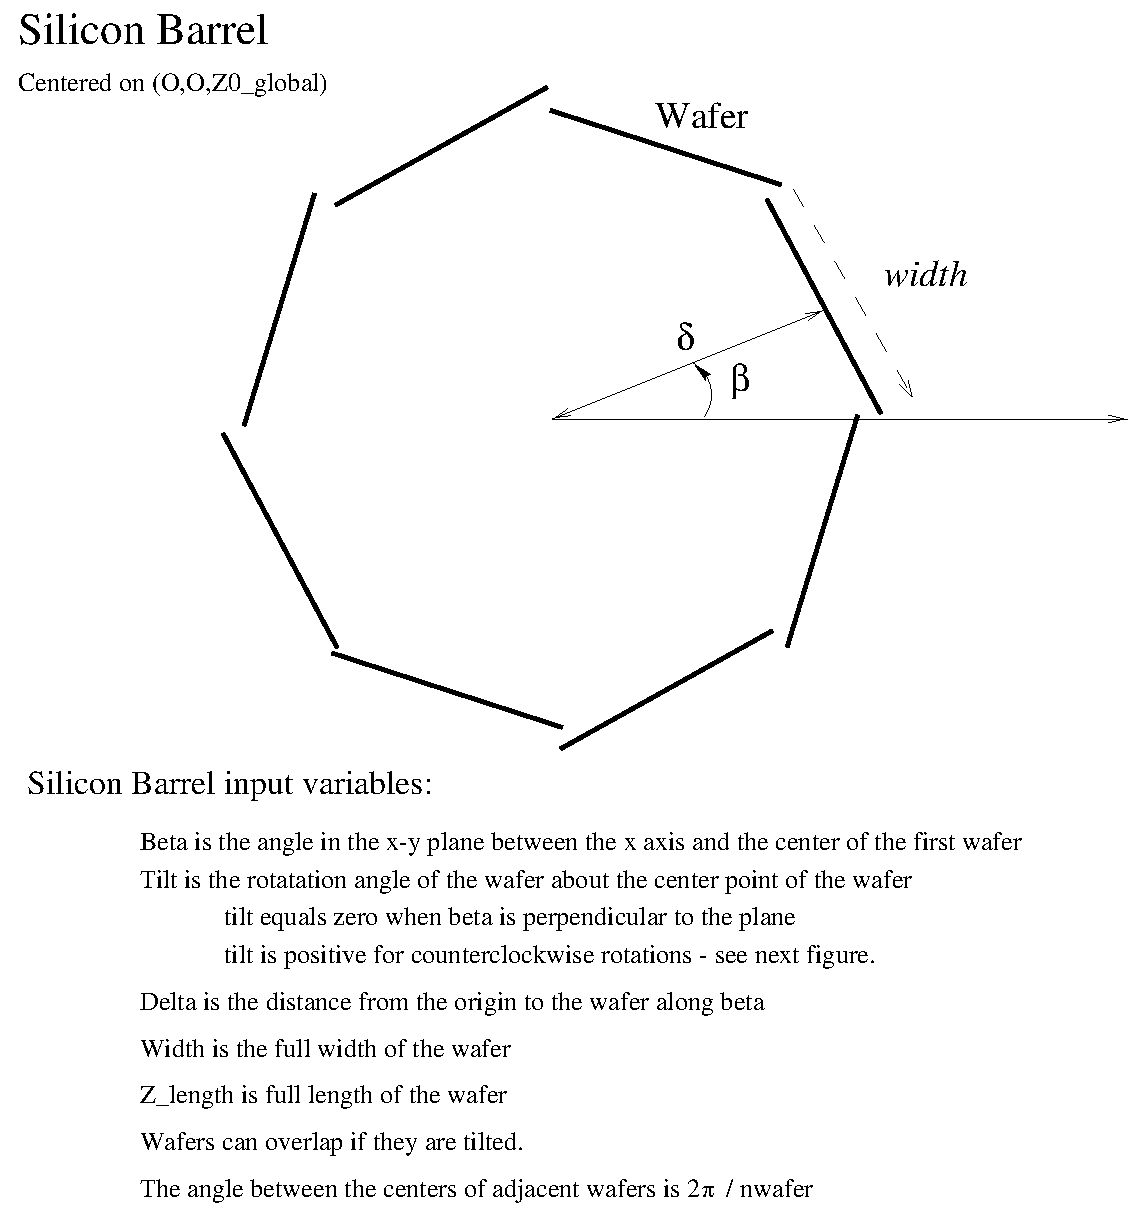
\psfig{file=sib.eps,width=7.5cm}}
\caption{\label{sib1} Silicon Barrel description, part 1 of 3.
See the next figure for an important caveat about $\beta$.
}

\end{figure}

\begin{figure} [htbp]
\centerline{\epsfxsize=5.0in \epsffile{LayerSiB_tilt.eps}}
%\centerline{
%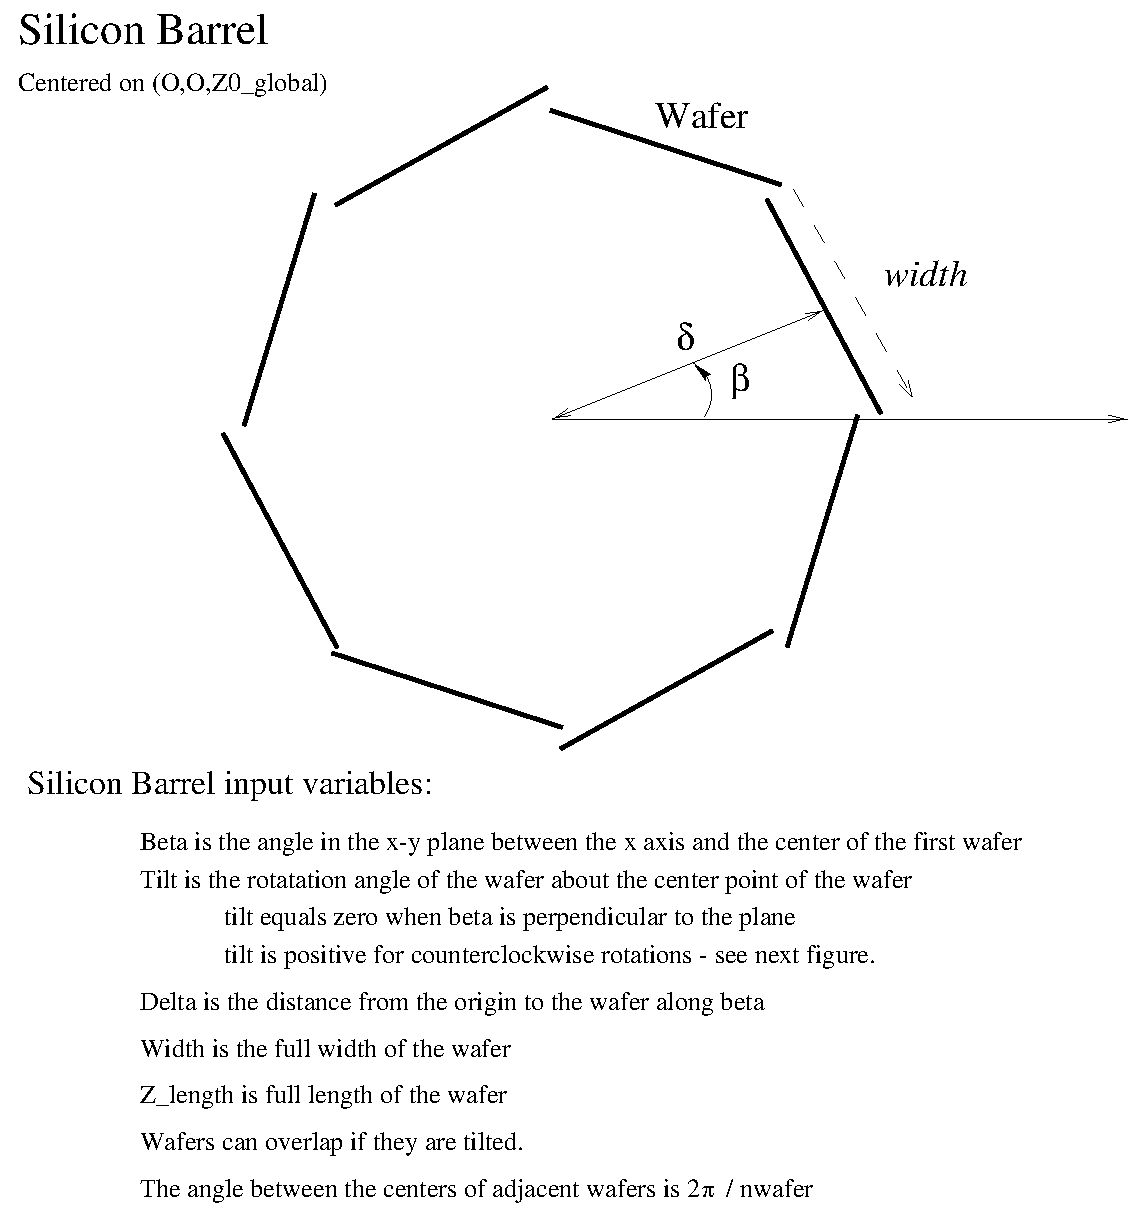
\psfig{file=sib.eps,width=7.5cm}}
\caption{\label{sib2} Silicon Barrel description, part 2 of 3.
This figure shows additional elements found in the db file.  It also
shows some of the derived quantities which are stored in the 
silicon barrel and rplane include files.}
\end{figure}



\begin{figure} [htbp]
\centerline{\epsfxsize=5.0in \epsffile{sibarrel_tree_db.eps}}
%\centerline{
%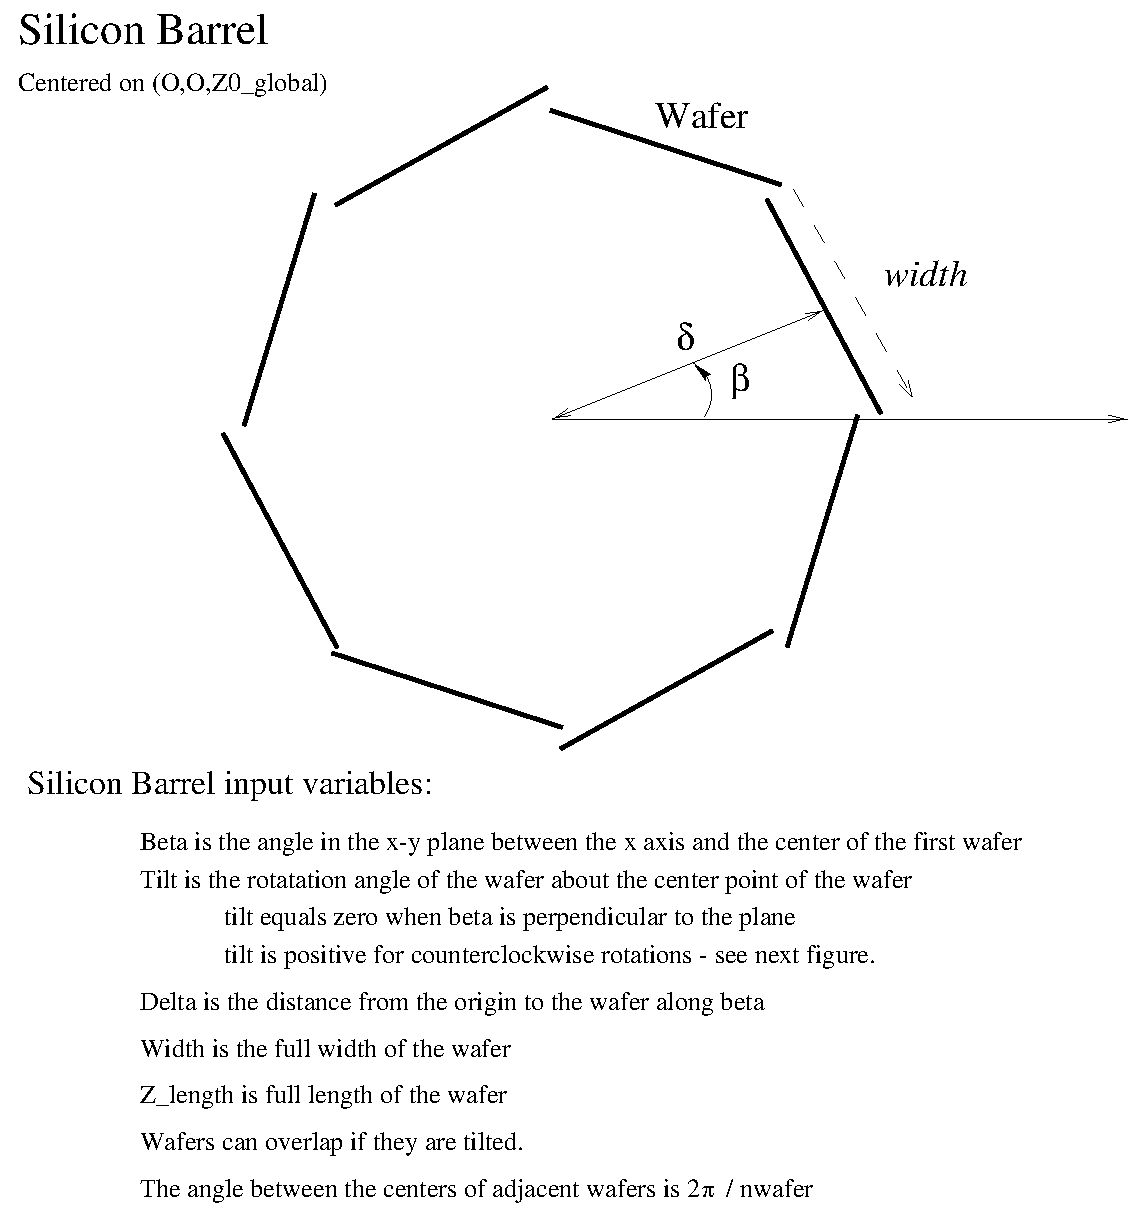
\psfig{file=sib.eps,width=7.5cm}}
\caption{\label{sib3} Silicon Barrel description, part 3 of 3.
This figure shows a graphical representation of the various elements
of the description of a silicon barrel detector.}
\end{figure}

Silicon Barrel layers:

\begin{itemize}
\item Siblayers
Layers for Silicon Barrel
\begin{description}
\item[{\rm template} LayerSiB](Max=30 total,  max 30 per device)  
\begin{description}
\item[{\rm  int} det]
\item[{\rm  parent} SiBarrel]
\item[{\rm  int} lyr]
\item[{\rm  material} mat]   material of layer
\item[{\rm  int} nwaf]       number of wafers in layer
\item[{\rm  child} Wafer]
\item[{\rm  real} zlen]      full length in Z  -- all wafers in one layer have
the same length
\item[{\rm  real} beta]      phi angle from the x axis to the center of wafer(1)
in the xy plane
\item[{\rm  real} delta]     radial distance in x-y plane to the center of each wafer 
\item[{\rm  real} thick]     layer thickness
\item[{\rm  real} width]     width of each wafer -- wafers can overlap
\item[{\rm  int} type]       type == 1= r/phi or stereo, 2 = z measurement
only;     you can use STEREO angle instead of type = 2
\end{description}
\item[end template]
\item[include file] \$MCFAST\_DIR/inc/geom/sib\_lyr\_struct.inc 
\end{description}

Silicon Barrel Wafers:

\begin{itemize}
\item Wafer \\

Planes (or Wafers) that make up the layers in a silicon barrel detector.
Wafers can overlap inside each layer. 
  

\begin{description}
\item[{\rm template} Wafer](Max=200 total in db file, Max = 110 per layer)
\begin{description}
\item[{\rm  char} speci]
\item[{\rm  int} det]
\item[{\rm  parent} LayerSiB]  Parent structure
\item[{\rm  int} lyr]       Parent layer
\item[{\rm  int} nwaf]      used only for speci=SPC, but ALWAYS present.
\item[{\rm  real} tilt]     positive tilt is counterclockwise
\item[{\rm  int} nstrip]    number of strips in layer 
\item[{\rm  real} c0x]      distance from midpoint of wafer
to strip number 0  (measured quantity corresponding to strip 0 in local
coordinates)
\item[{\rm  real} x0y]      needed for z measurement-- type = 2
\item[{\rm  real} pitch]    pitch of strips
\item[{\rm  real} stereo]   stereo angle in radians of strips -- relative to $\phi$
measurement 
\item[{\rm  real} eff\_hit]
\item[{\rm  real} siga]  resolution in cm -- see below
\item[{\rm  real} sigb]
\item[{\rm  real} sigc]
\end{description}
$      \sigma = \sigma_a
           + \sigma_b \times |\cos \theta|
           + \sigma_c \times cos^2 \theta  $ \\
$     \cos\theta = pz/p$
\item[end template]
\item[include file] \$MCFAST\_DIR/inc/geom/sib\_plane\_struct.inc 
\end{description}
\end{itemize}
\end{itemize}

\filbreak

\subsection{Silicon forward disks}
Silicon forward disks are described by layers of non-overlapping wedges. 
(See figures~\ref{sidisk}, ~\ref{sid_type} and~\ref{wedge_coord}.)
The disks are perpendicular to the $z$ axis.  

\begin{description}
\item[{\rm template} SiDisk](Max=32)  
\begin{description}
\item[{\rm  int} num]
\item[{\rm  char} name]
\item[{\rm  int} nlyr]
\item[{\rm  real} zpos]  Z position of detector
\end{description}
\item[end template]
\item[include file] \$MCFAST\_DIR/inc/geom/sicir\_disk.inc, sicir\_disk\_struct.inc 
\end{description}

\begin{figure} [htbp]
\centerline{\epsfxsize=6.0in \epsffile{sidisk.eps}}
\caption{\label{sidisk} Silicon Disk description}
\end{figure}

Layers in Silicon Disks Detectors:

\begin{itemize}
\item Sidisk\_layer  \\
Layers that make up the forward disk detectors
\begin{description}
\item[{\rm template} LayerSiDi](Max=80 , max = 80 per device)
\begin{description}
\item[{\rm  int} det]       pointer to SiDisk device number
\item[{\rm  parent} SiDisk] Parent structure
\item[{\rm  int} lyr]       layer number
\item[{\rm  material} mat]  material (``SILI'' for example)
\item[{\rm  int} nwed]      number of wedges in this layer
\item[{\rm  child} Wedge]   Wedge structure
\item[{\rm  real} z\_local]  z of layer relative to detector Z position
\item[{\rm  real} thick]    thickness of silicon in layer
\item[{\rm  real} rmin]     minimum radius (for type 1-3; distance to edge for type 4)
\item[{\rm  real} rmax]     maximum radius (for type 1-3: distance to edge for type 4)
\item[{\rm  real} phi(2)]   $\phi$ coverage of layer (0,2$\pi$) for full coverage
\item[{\rm  real} dphi]   $\phi$ coverage of one wedge: 
$(\phi(2)-\phi(1))/\rm nwed$ for full coverage
with no gaps.  First wedge is centered at $\phi(1) + (\phi(2)-\phi(1))/2\rm  nwed$
\item[{\rm  int} type]    measurement type  \\
                                 1 r measurement -- code under development \\
                                 2 phi measurement \\
                                 3 U/V measurements-- radial edges at rmin/rmax \\
                                 4 U/V measurements-- straight edges at rmin/rmax\\                                 
\end{description}
\item[end template]
\item[include file] \$MCFAST\_DIR/inc/geom/sicir\_lyr\_struct.inc 
\end{description}

\begin{figure} [htbp]
\centerline{\epsfxsize=6.0in \epsffile{sid_type.eps}}
\caption{\label{sid_type} Silicon Disk Types}
\end{figure}

Wedges of silicon disk layers:

\begin{itemize}
\item Sidisk\_wedge  \\
Wedges in one layer cannot overlap.
Strip number is calculated relative to an outer corner of the disk and should be positive.
For positive stereo (0 $<$ stereo $<$ $\pi/2$) nstrip counts from the outer corner at low phi.
\begin{description}
\item[{\rm template} Wedge](Max=80 total in db file, Max= 80 per layer)
\begin{description}
\item[{\rm  char} speci]         ``SPC'' do define each one or ``ALL'' for all
\item[{\rm  int} det]     SiDisk number
\item[{\rm  parent} LayerSiDi] Parent structure
\item[{\rm  int} lyr]    layer number
\item[{\rm  int} nwed]   wedge number: only used for speci=``SPC'', but ALWAYS present
\item[{\rm  int} nstrip] number of strips on wedge
\item[{\rm  real} c0\_r] -- width of dead region in R\\
--  will make symmetric dead regions at inner and outer edge
\item[{\rm  real} c0\_phi] -- width of dead region in phi\\
-- will make symmetric dead regions at phi edges
\item[{\rm  real} pitch]  strip pitch  
\item[{\rm  real} stereo] stereo angle in radians-- for type 3 and 4 only
\item[{\rm  real} eff\_hit]  hit efficiency
\item[{\rm  real} siga]  -- type 2 in radians
\item[{\rm  real} sigb]  
\item[{\rm  real} sigc] 
$\sigma = \sigma_a$ in cm for type 3-4, in radians for type = 2
\end{description}
\item[end template]
\item[include file] \$MCFAST\_DIR/inc/geom/sicir\_wedge\_struct.inc
\end{description}
\end{itemize}
\end{itemize}

At present only siga is used in trk\_make\_sidisk\_hit.F.
\filbreak

\begin{figure} [htbp]
\centerline{\epsfxsize=4.5in \epsffile{wedge_coord.eps}}
\caption{\label{wedge_coord} Coordinate systems for forward silicon
detectors of wedge type 4. The figure shows cartoons of three wedges
in the $xy$ plane.  The point labeled O is the beam spot.
The dashed lines show the center lines of the wafers.
The solid lines show several of the sense strips on the wafers.
The curved arrow on wedge 1 shows the sense of a positive stereo angle,
clockwise wrt the center line; wedge 1 shows an example
of a positive stereo angle and wedge 2 shows an example of a negative
stereo angle. Wedge 3 shows a stereo angle of $+90^{\circ}$.  
The point A and the arrow attached to it show the origin of the coordinate
system and the positive sense of measurements for wedge 1.  Similarly
the points B and C show, respectively, the origins and positive sense
for wafers 2 and 3.
}
\end{figure}


\subsection{Silicon planes (xy)}

Planar Silicon detectors are described by rectangular surfaces 
perpendicular to the $z$ axis. These detectors can be strips or pixels.
MCFast provides two device types to describe such planes,
{\tt SiXY} devices and {\tt SiZRect} devices.  The former device type is
the simpler of the two and is described in this subsection.  The latter
is more general and is described in the next subsection.

\begin{description}
\item[{\rm template} SiXY](Max=100)
\begin{description}
\item[{\rm  int} num]  station number
\item[{\rm  char} name]  station name
\item[{\rm  int} nly]   number of layers in each station
\item[{\rm  child} LayerSiXY]
\item[{\rm  real} zpos]  z position of station
\end{description}
\item[end template]
\item[include file] \$MCFAST\_DIR/inc/geom/sixy\_disk.inc, sixy\_disk\_struct.inc 
\end{description}
Silicon $xy$ plane layers:
\begin{itemize}
\item Sixy\_layer
\begin{description}
\item[{\rm template} LayerSiXY](Max = 500 total, max = 100 per device)
\begin{description}
\item[{\rm  int} det]   station id
\item[{\rm  parent} SiXY]
\item[{\rm  int} lyr]   layer id
\item[{\rm  material} mat]   material
\item[{\rm  real} z\_local]  local z position relative to station position
\item[{\rm  real} thick]     layer thickness
\item[{\rm  real} stereo]    stereo
\item[{\rm  int} type]       type
\item[{\rm  real} eff\_hit]  efficiency
\item[{\rm  real} xmin]      x min of layer
\item[{\rm  real} xmax]      x max of layer
\item[{\rm  real} xmin\_gap] x min of gap
\item[{\rm  real} xmax\_gap] x max of gap
\item[{\rm  int} nsegm\_x]   number of strips or pixels in x
\item[{\rm  real} pitch\_x]  pitch of pixels in x
\item[{\rm  real} coord0\_x] local coordinate 0 for x
\item[{\rm  real} sigma\_x]  resolution in x ( see below for negative values)
\item[{\rm  real} ymin] y min of layer
\item[{\rm  real} ymax] y max of layer
\item[{\rm  real} ymin\_gap] u min of gap
\item[{\rm  real} ymax\_gap] y max of gap
\item[{\rm  int} nsegm\_y]  number of segments in y
\item[{\rm  real} pitch\_y] pitch in y
\item[{\rm  real} coord0\_y] local coordinate 0 for y coordinate
\item[{\rm  real} sigma\_y]  resolution in y ( see below for negative values)
\end{description}
\item[end template]
\item[include file] \$MCFAST\_DIR/inc/geom/sixy\_disk\_layer\_struct.inc 
\end{description}
\end{itemize}

If either sigma\_x or sigma\_y is negative, then the user
routine usr\_siz\_rect\_res.F will be called to compute the
measurement and the error on the measurement.  This hook can be
used, for example, to generate clusters of hit strips rather
than just throwing a gaussian resolution.

It is not possible to declare rotated sixy layers;
this functionality, however, is provided for SizRect devices,
which are described in the next subsection.
\filbreak

\subsection{Silicon Rectangular Z-Planes (SiZRect)} 
Planar Silicon detectors 
can also be described by rectangular surfaces (silicon wafers) perpendicular 
to z axis but not necessarily centered about z axis.
One more wafers forms a layer and one or more layers forms a station. 
For the purpose of tracking, wafers are treated as infinitesimally
thin objects. However the description of the wafer does include a thickness,
which is only used in the computation of the expected multiple scattering
and energy loss; these are applied as if they occured at the infinitesimally
thin plane. 

\begin{description}
\item[{\rm template} SizRect] (Max=100) 
\begin{description}
\item[{\rm int} num]  station number 
\item[{\rm char} name] station name 
\item[{\rm int} nlayers] number of layers in the station 
\item[{\rm child} LayerSizRect ] 
\item[{\rm real} xpos] x-position of station's center (in global 
coordinate system) 
\item[{\rm real} ypos] y-position of station's center (in global 
coordinate system) 
\item[{\rm real} zpos] z-position of station's center (in global 
coordinate system) 
\end{description}
\item[end template] 
\item[include file] \$MCFAST\_DIR/inc/geom/siz\_rect.inc,
siz\_rect\_struct.inc 
\end{description}

{\bf Silicon rectangular layers:} \\
Layers that make up the rectangular silicon detectors.  A layer may have
a rectangular inner gap. The center of the gap must coincide with
the center of layer.
Three types of gaps are supported, X, Y, and window; these
are illustrated in figure~\ref{siz1}.
A layer may be rotated about the z axis. 
For a layer with a window-type gap, wafers are not permitted to
overlap each other.  For all other gap types, including no gap,
wafers within a layer may overlap in x and/or y.
The MCFast wafer numbering convention is that the wafer 1 is in the
upper left corner of the layer.  Wafer numbers then increase across the 
layer in x and then down in y.  Wafers may be offset from the average
z-position of the layer; see~figure~\ref{siz2} and the
description of wafers, below.

\filbreak

\begin{itemize}
\item Siz\_rect\_layer
\begin{description}
\item[{\rm template} LayerSizRect] (Max=500, max=20 per device) 
\begin{description}
\item[{\rm int} det] station id 
\item[{\rm parent} SizRect] 
\item[{\rm int} lyr] layer id 
\item[{\rm int} nWaferX] number of segments along x-direction  
\item[{\rm int} nWaferY] number of segments along y-direction  
\item[{\rm real} zLayerLocal] local z-position of layer relative 
to station position 
\item[{\rm real} rotation] rotation of layer about z axis;
                           see text for details.
\item[{\rm real} Xlen] layer full length along x  
\item[{\rm real} Ylen] layer full length along y  
\item[{\rm real} GapXlen] full width along x of gap in layer (see note below)  
\item[{\rm real} GapYlen] full width along y of gap in layer (see note below) 
\item[{\rm char} StaggeringPattern] X, Y, CH, or NONE. See below.
\end{description}
\item[end template] 
\item[include file] \$MCFAST\_DIR/inc/geom/siz\_rect\_layer\_struct.inc
\end{description}
\end{itemize}
%
A full description of the staggering pattern is given after the
wafer template has been described.

To implement a gap one should specify:
\begin{description}
\item[X:] {\bf GapXlen$>$0  \&\& GapYlen=Ylen}
\item[Y:] {\bf GapXlen=Xlen \&\& GapXlen=Xlen}
\item[Window:]{\bf 0$<$GapXlen$<$Xlen \&\& 0$<$GapYlen$<$Ylen}.
\end{description}

\filbreak

\begin{figure} [htbp]
\begin{center}
\centerline{\epsfysize=3.0in \epsffile{sizRectGaps.eps}}
\caption{\label{siz1} Rectangular Silicon Layers with Gaps (front view)}
\end{center}
\end{figure}

\filbreak

{\bf Silicon rectangular wafers:}
\begin{itemize}
\item{Siz\_rect\_wafer}
\begin{description}
\item[{\rm template} WfrSizRect] (Max=500, max=200 per layer) 
\begin{description}
\item[{\rm char} speci] ALL, SPC or ONE; see below.
\item[{\rm int} det] station id 
\item[{\rm parent} LayerSizRect] 
\item[{\rm int} lyr] layer id 
\item[{\rm int} waferX] wafer id along x (in layer coordinate system); ignored
for speci=ALL; should be non-zero for speci=SPC. 
\item[{\rm int} waferY] wafer id along y (in layer coordinate system); ignored
for speci=ALL; should be non-zero for speci=SPC.
\item[{\rm int} type] 1=pixel, 2=strips 
\item[{\rm material} mat] material (for example, "SILI")
\item[{\rm real} eff\_hit] efficiency 
\item[{\rm real} stereo] orientation of strips wrt x axis; see below.
\item[{\rm real} Xlen] length of wafer along x 
\item[{\rm real} Ylen] length of wafer along y 
\item[{\rm real} Zlen] z-thickness of wafer 
\item[{\rm real} zOffset] $z$ offset for staggering pattern. See below.
\item[{\rm int} nsegm\_x] number of strips or pixels along x 
\item[{\rm real} pitch\_x] pitch of strips of pixels in x 
\item[{\rm real} coord0\_x] local coordinate of first strip of pixel for x 
\item[{\rm real} sigma\_x] resolution in x (see below for negative values)
\item[{\rm int} nsegm\_y] number of strips or pixels along y 
\item[{\rm real} pitch\_y] pitch of strips of pixels in y 
\item[{\rm real} coord0\_y] local coordinate of first strip of pixel for y 
\item[{\rm real} sigma\_y] resolution in y (see below for negative values)
\end{description}
\item[end template] 
\item[include file] \$MCFAST\_DIR/inc/geom/siz\_rect\_wafer\_struct.inc
\end{description}
\end{itemize}

This template describes wafers which make up layers.
If {\tt speci=ALL} then MCFast will fill the layer with copies
of this wafer definition; this is done according to nWaferX, nWaferY,
the gap size and the staggering pattern, all of which 
are defined in the layer template.  If any part of a wafer intrudes
into the gap, it is omitted from the pattern.  Also

If {\tt speci=SPC} then this wafer definition is used to define 
exactly one wafer, the one specified by waferX and waferY.
If a layer is composed of some repeated wafers 
plus a few special ones, the {\tt speci=ALL} wafer must appear 
first in the {\tt .db} file, followed by the {\tt speci=SPC} wafer(s).

With v5\_0 there is a new value, {\tt speci=ONE}.
Wafers with this value are treated the same as ALL 
except that the wafers are permitted to overlap the central gap/hole; 
this value of speci can be used to clone sixy devices by making layers
with one big wafer.

For {\tt speci=ALL} wafers, the z-position of the center of wafer 1, 
relative to the nominal z of the layer, is specified by the 
zOffset parameter.  See figure~\ref{siz2}.  The
z-positions of the remaining wafers in the layer are calculated 
using zOffset and the StaggeringPattern specified for that layer.
%
\begin{figure} [htb]
\begin{center}
\centerline{\epsfysize=3.0in \epsffile{sizRectWafers.eps}}
\caption{\label{siz2} Offset Silicon Wafers (side view)}
\end{center}
\end{figure}
%
The staggering patterns are:
%
\begin{description}
   \item[X] The first {\bf column} is offset by {\tt +zOffset}, the second
             by {\tt -zOffset}, $\dots$; that is, the pattern alternates 
             in X.
   \item[Y] The first {\bf row} is offset by {\tt +zOffset}, the second
             by {\tt -zOffset}, $\dots$; that is, the pattern
             alternates in Y.
   \item[CH] A checkered board pattern.  The wafer in the upper left
             corner is offset by {\tt +zOffset}, its lower and right
             neighbours are both offset by {\tt -zOffset}, and so on.
   \item[NONE] All wafers in the layer are at {\tt +zOffset}.
\end{description}
%
In case of {\tt speci=SPC} the wafer z-position is defined directly by 
zOffset.


If either sigma\_x or sigma\_y is negative, then the user
routine usr\_siz\_rect\_res.F will be called to compute the
measurement and the error on the measurement.  This hook can be
used, for example, to generate clusters of hit strips rather
than just throwing a gaussian resolution.

Figures~\ref{siz3} and~\ref{siz4} show the meaning of some of the
parameters used to position wafers within a layer.  In particular,
figure~\ref{siz3} makes the distinction between rotation angles and
stereo angles.  For convenience, all of the positioning parameters,
except for the rotation angle itself, are defined for an unrotated layer.
In figure~\ref{siz4} the outer rectangle marks the physical size of
the wafer while the inner rectangle marks the active area of the wafer;
the widths of the horizontal and vertical dead areas are
allowed to be different.   The active area is centered on the full 
area of the wafer.  The point marked $(x_0,y_0)$ corresponds to 
{\tt (coord0\_x,coord0\_y)}, which defines the lower left hand 
corner of the active area.


\begin{figure} [htbp]
\begin{center}
\centerline{\epsfysize=3.0in \epsffile{sizRectAlign.eps}}
\caption{\label{siz3} This figure shows the stereo angle, $\theta_s$,
                      which is defined in the wafer template,
                      and the rotation angle, $\theta_R$,
                      which is defined in the layer template.}
\centerline{\epsfysize=3.0in \epsffile{sizRectOrigin.eps}}
\caption{\label{siz4} The left hand figure shows a wafer in an unrotated
position while the right hand figure shows the same wafer in its
rotated position.   For convenience, the positioning parameters
are defined in the unrotated configuration.}
\end{center}
\end{figure}

The points marked $(x_1,y_1)$ and the vector $\vec{\eta}$ are of
concern only to experts.  These are defined similarly to the
corresponding quantities for forward tracking detectors.

\subsubsection{Stereo angles for SiZRecT Devices}

There are some restrictions when specifying stereo
angles for SizRect devices.  

As of version v5\_0, stereo angles and rotation angles only
work properly for strip SizRect devices.  Pixel devices must
have {\tt stereo=0.0} and {\tt rotation=0.0}.  This will
be fixed in a future release.

It is necessary that 
the dimensions of the active area, the pitch and the number of
pixels in each dimension be self consistent.  MCFast does not
check for this.

There is a special case which is important.  If one specifies, 
{\tt nsegm\_x$>$1}, {\tt nsegm\_y=1} and {\tt stereo=0}, then
MCFast will assume that the user really intended to measure
the local $x$ coordinate; therefore the routine which makes
SizRect hits will use {\tt stereo=-$\pi$/2}.
Without this trick, the user would have to specify a lot of digits in 
{\tt stereo} in order to get a true $x$ measurement.

For a general stereo angle, 
it is required that {\tt nsegm\_x$>$1}.  If one specifies
{\tt nsegm\_x=1}, {\tt nsegm\_y$>$1} and {\tt stereo$\ne$0.0},
the program will print an error message and stop.
See the discussion on stereo angles in subsection~\ref{sec:ftrk}
for for the algebra needed to keep 
{\tt nsegm\_x} and {\tt pitch\_x} consistent with the dimensions
of the active area.  In addition figure~\ref{ftrk6} may be useful.


\filbreak


\subsection{Solenoid magnet}
\begin{description}
\item[{\rm template} Solenoid](Max=10)
\begin{description}
\item[{\rm char} name]    Name
\item[{\rm real} bfield]  Magnitude of B -field
\item[{\rm  real} rmin]   minimum radius of solenoidal field (should be 0.0)
\item[{\rm  real} rmax]   maximum radius of solenoidal field
\item[{\rm  real} z0]     Central z position of field region
\item[{\rm  real} zlen]   length in Z
\item[{\rm  material} mat\_fill]  material inside solenoid (not used)
\item[{\rm  real} thick\_boun(4)]    boundary thickness at rmin=0 , rmax(coil), zmin =0, zmax =0  
\item[{\rm  material} mat\_boun(4)]  material at boundary  rmin=' ', rmax(coil material), zmin=' ', zmax=' '
\end{description}
\item[include file] \$MCFAST\_DIR/inc/geom/solenoid.inc 
\item[end template]
\end{description}



\newpage
\section{The Include files}

\subsection{Silicon barrel detectors}  
\label{page:sib:include}
The include files listed 
below show the structures which describe a silicon barrel detector;
see figures~\ref{sib1} and~\ref{sib2}.  Recall that the parameter
$\beta$ means one thing in the .db file and another in the
data structures below.  ( The description of the .db file begins
on page~\pageref{page:sib:detectors}. )  Finally, figure~\ref{sib4} shows
the relationships between the structures which describe a complete
silicon barrel detector.


\begin{description}
\item[include file:] \$MCFAST\_DIR/inc/geom/si\_barrel.inc,
si\_barrel\_struct.inc
\item[{\rm structure /si\_barrel\_struct/}] (Max=15)
\begin{description}
\item[{\rm integer}  numlyr] Number of layers
\item[{\rm integer} nchan]   Total number of channels
\item[{\rm record /sib\_lyr\_struct/} lyr(max\_sib\_lyr)] Layer parameters
\item[{\rm character*40} name] Name of device
\item[{\rm real} z] Global z-position of center of device
\end{description}
\item[end structure]
si\_barrel\_struct.inc 
\item[template file:] \$MCFAST\_DIR/db/sibarrel.db
\end{description}


\begin{description}
\item[include file:] \$MCFAST\_DIR/inc/geom/sib\_lyr\_struct.inc 
\item[{\rm structure /sib\_lyr\_struct/}] (Max=30)
\begin{description}
\item[{\rm integer} numplane] Number of planes in the layer
\item[{\rm integer} nchan] Number of channels in this layer
\item[{\rm integer} chan0] Channel number of 1st strip
\item[{\rm record /sib\_plane\_struct/} plane(max\_sib\_plane)]
  Parameters of each plane in the layer
\end{description}
\item[end structure]
\item[template file:] \$MCFAST\_DIR/db/siblayers.db
\end{description}


\begin{description}
\item[include file:] \$MCFAST\_DIR/inc/geom/sib\_plane\_struct.inc 
\item[{\rm structure /sib\_plane\_struct/}]  (Max=110)
\begin{description}
\item[{\rm integer} type] 1 = r-phi measurement;
				2 = z measurement
\item[{\rm real} dmin] dmin of plane (in r-phi direction)
\item[{\rm real} dmax] dmax of plane (in r-phi direction)
\item[{\rm real} zmin] zmin of plane
\item[{\rm real} zmax] zmax of plane
\item[{\rm real} beta] Angle between normal to plane and x axis
\item[{\rm real} xpos(3)] Center of wafer.
\item[{\rm real} eta(3)] Direction cosines of normal to plane
\item[{\rm real} delta\_min] Minimum distance from origin to edge of plane
\item[{\rm real} delta\_max] Maximum distance from origin to edge of plane
\item[{\rm real} thick] Thickness of plane
\item[{\rm real} tilt] Tilt angle for plane
\item[{\rm real} eff\_hit] Hit efficiency
\item[{\rm real} siga] Constant a in resolution formula
\item[{\rm real} sigb] Constant b in resolution formula
\item[{\rm real} sigc] Constant c in resolution formula
\item[{\rm integer} material] Material composing plane
\item[{\rm real} coord0\_x] Local x-coordinate of strip 0
\item[{\rm real} coord0\_y] Local y-coordinate of strip 0
\item[{\rm real} pitch] Spacing of strips
\item[{\rm integer} nstrip] Number of strips in this plane
\item[{\rm integer} nchan] Number of channels in this plane
\item[{\rm integer} chan0] Channel number of the 1st strip in plane
\item[{\rm real} stereo] Stereo angle in rad
\item[{\rm real} cos\_stereo] cos(stereo)
\item[{\rm real} sin\_stereo] sin(stereo)
\end{description}
\item[end structure]
\item[template file:] \$MCFAST\_DIR/db/wafer.db
\end{description}



\begin{figure} [htbp]
\centerline{\epsfxsize=5.0in \epsffile{sibarrel_tree_1.eps}}
%\centerline{
%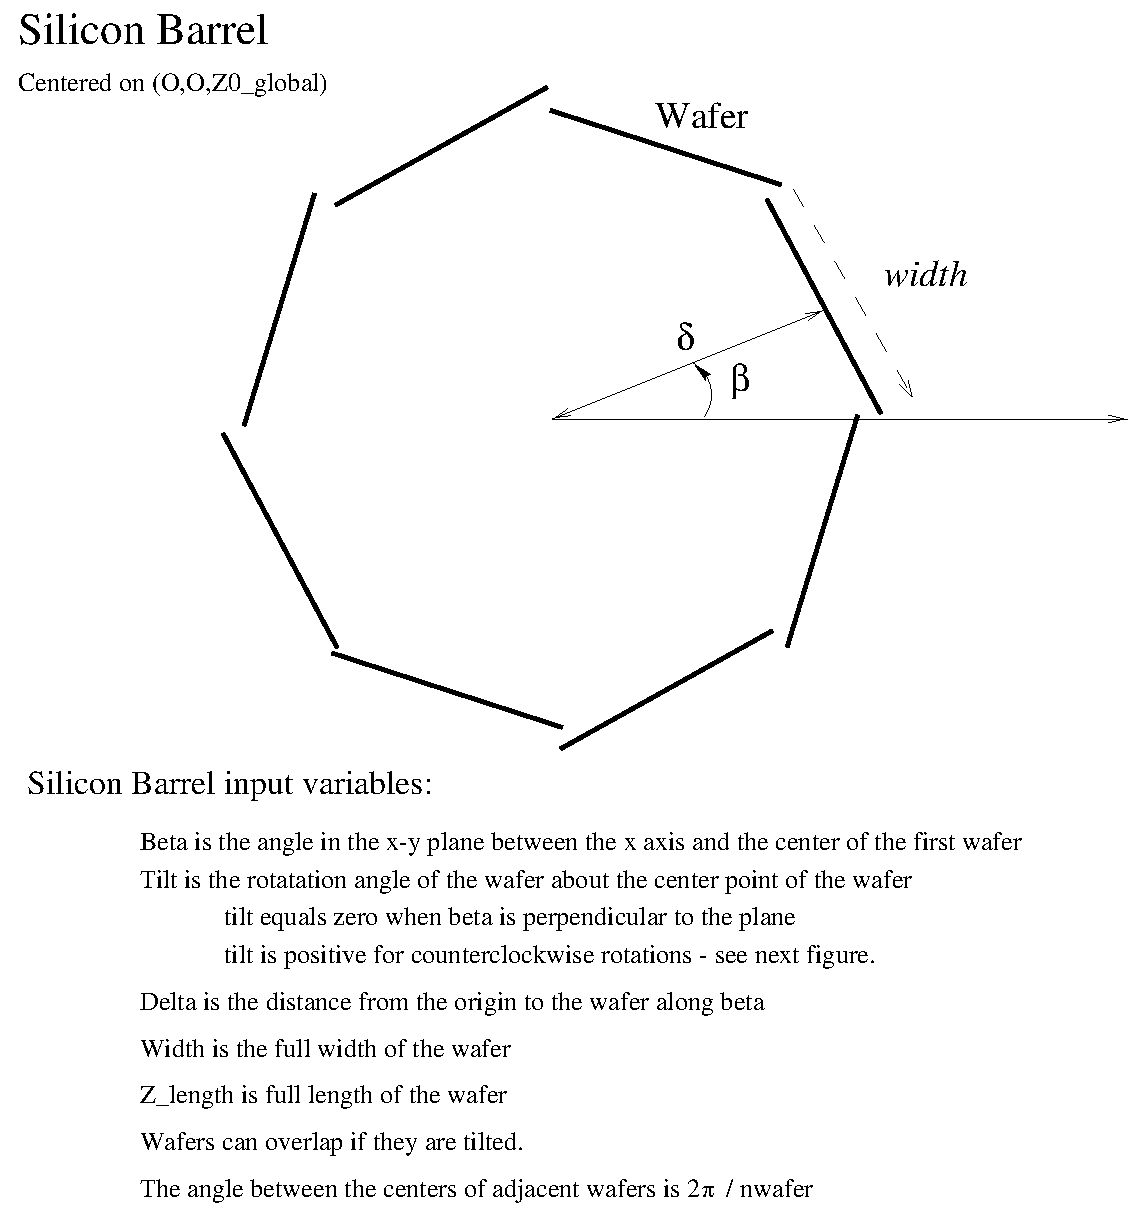
\psfig{file=sib.eps,width=7.5cm}}
\caption{\label{sib4} Silicon Barrel description. This figure shows
the relationships between the elements which describe a silicon
barrel detector.}
\end{figure}


\end{document}



